\documentclass[11pt]{article}
\usepackage{amsmath,amssymb, amsthm, marvosym, permute, extsizes}
\usepackage{siunitx, graphicx, float, enumitem, adjustbox, hyperref, bm, bbm}
\usepackage{microtype, dsfont}
\usepackage[normalem]{ulem}
\usepackage[T1]{fontenc}
\usepackage[utf8]{inputenc}
\usepackage{lmodern}
\usepackage{moreenum}
\usepackage{braket, bbold}
\usepackage[T1]{fontenc}
\usepackage[a4paper,margin=2.5cm]{geometry}
\usepackage[icelandic]{babel}
\def\rcurs{{\mbox{$\resizebox{.09in}{.08in}{\includegraphics[trim= 1em 0 14em 0,clip]{ScriptR}}$}}}
\def\brcurs{{\mbox{$\resizebox{.09in}{.08in}{\includegraphics[trim= 1em 0 14em 0,clip]{BoldR}}$}}}
\usepackage{tikz}
\usepackage{pdfpages}
\usepackage{todonotes}
\newcommand{\explain}[2]{\underbrace{#1}_\textrm{$#2$}}
\newcommand{\angstrom}{\textup{\AA}}

\title{Greining á flogaköstum í heilaritum\\ \Large{ Gervigreind}}
\author{Alexander Guðjónsson \and Emil Gauti Friðriksson }
\date{\vspace{-1ex}Apríl 2019}
\begin{document}
\maketitle
\section{Inngangur}
Viðfangsefni þessarar skýrslu er greining EEG heilarita og þá sérstaklega hvernig greina má mun heilarita einstaklinga með flog og án floga. Mynd \ref{fig:flog} sýnir dæmi um heilbrigt heilrit og flogakast. Fundin voru ýmis auðkenni gagnanna og út frá þeim voru þjálfaðir og fínstilltir þrír flokkarar: Stoðvigravél, lógistísk aðhvarfsgreining og AdaBoost. Flokkurunum var síðan beitt í einstaklingsmiðuðu mati, þá er þjálfaður flokkari á gögnum allra sjúklinganna nema þanns einstaklings sem flokkarinn er síðan prófaður á. Ásamt flokaranna þriggja þá var einnig smíðað tauganet út frá rófriti EEG mælinganna.\\
\begin{figure}[H]
    \centering
    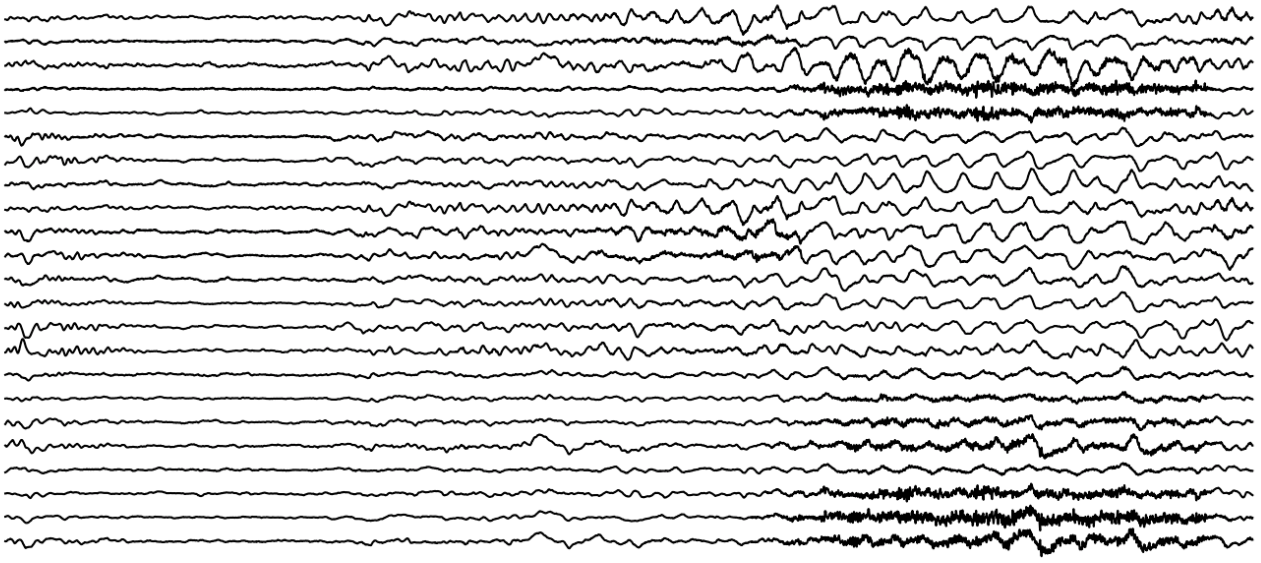
\includegraphics[height=50mm]{flog.PNG}
    %\caption{flog}
    \label{fig:flog}
\end{figure}
\begin{figure}[H]
    \centering
    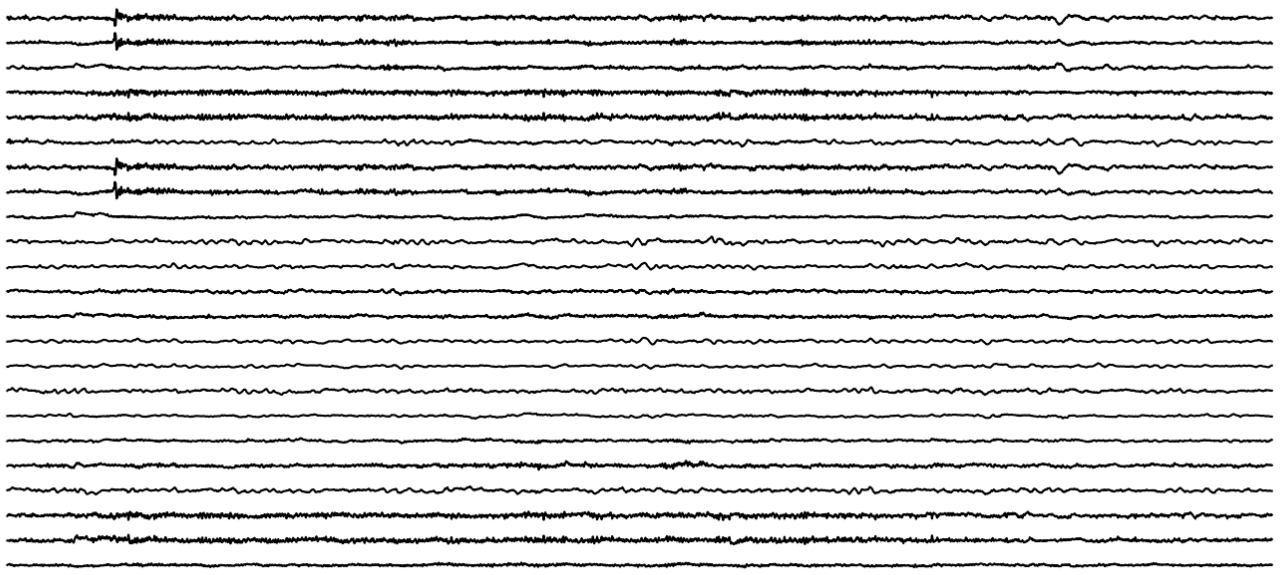
\includegraphics[height=50mm]{ekkiFlog.PNG}
    \caption{Heilarit af flogi (uppi) og heilbrigt heilarit (niðri)}
    \label{fig:ekkiFlog}
\end{figure}
%Hvað var gert, hvers vegna  og hvernig


Sjálfvirk greining EEG heilarita hvort það sýni flog eða ekki gæti orðið verðmætt verkfæri lækna og sjúklinga þeirra sem þjást af flogum. Enn í dag þurfa sérfræðingar oft að rýna í heilarit handvirkt til að greina hvort um hafi verið að ræða flog eða ekki. Þetta er kjörið verkefni fyrir vélnám og gervigreind því magn gagna sem safnast er oft mjög mikið.


\section{Aðferðir}
\subsection{Gögn}
Gögn notuð í þessu verkefni voru fengin úr doktorsverkefni Ali Shoeb\cite{Doctorsgrein} úr MIT. Gögnin samanstanda af 14 sekúnda heilaritum flokkuð eftir hvort þau sýni flog eða ekki. Safnað hefur verið saman 170 flogamælingum og 370 mælingum án floga, samtals 540 mælingum. Hver þessara 540 mælinga inniheldur svo 23 tímaraðir. Mælingar eru teknar með svokölluðu 10-20 kerfi\cite{EEG-maeling}.
\subsection{Auðkenni}
Þegar litið er á tímaraðirnar sjálfar sem inntaksgögn þá eru þau alls ekki lýsandi enda liggur áhuginn ekki á einstökum gildum. Í tímaröðum sem lýsa heilaritum liggur áhuginn frekar á að skoða heildarmyndina út frá eiginleikum sem byggja á tíðni raðanna, kallaðir rófseiginleikar (e, spectral features). Í okkar greiningu reiknuðum við aflrófsþéttleika (e. power spectral density) fyrir mismunandi tíðnibönd (kölluð $\alpha, \beta, \delta, \theta$) og Hjorth gildi hverrar tímaraðar og notum þær stærðir frekar sem inntök í flokkarana okkar \cite{Hjorth}. 

Notast var við aðferð Welch's við þá reikninga sem má finna í {\tt signal} pakkanum hjá {\tt scipy}. Einn galli við þessar stærðir er að þær týna upplýsingum um tíma í röðunum en í heilaritum má gjarnan finna forboða fyrir flogaköstin svo við viljum geta nýtt upplýsingar um tíma í greiningu okkar. Við gerðum það með því að skipta tímaröðunum, sem eru 14 sekúndur niður í minni tímabil og skoða rófseiginleikana á hverju bili fyrir sig.
Við fundum bestu stærðina fyrir tímarammann með því að þjálfa flokkarana okkar á öllum mögulegum stærðum og bera saman prófunarnákvæmni þeirra.
\subsection{Flokkarar}
Við bárum saman þrjár gerðir flokkara, lógistíska aðhvarfsgreiningu, stoðvigravél og safnaðferðina AdaBoost. Allir þessir þrír flokkarar eru tvíkostaflokkarar (e. binary classifiers) og því vel við hæfi fyrir okkar verkefni.
\subsubsection{Lógistísk aðhvarfsgreining}
Í lógistískri aðhvarfsgreiningu smíðum við líkanið
$$ f_{\theta}(x)=\frac{1}{1+\exp (-\theta^{T} x)} $$
þar sem við ákvörðum stikana $\theta$ með því að hámarka logra sennileikafallið
\begin{equation}
    \log(L(\theta)) = \sum _ { i = 1 } ^ { n } y ^ { ( i ) } \log g \left( \theta ^ { T } x ^ { ( i ) } \right) + \left( 1 - y ^ { ( i ) } \right) \log \left( 1 - g \left( \theta ^ { T } x ^ { ( i ) } \right)\right).
\end{equation}
Flokkun gagnanna verður þá
$$ \hat{y}=\left\{\begin{array}{ll}{1} & {\text { ef } g\left(\theta^{T} \hat{x}\right) \geq 0.5} \\ {0} & {\text { annars }}\end{array}\right. $$
Við notum {\tt LogisticRegression} fallið úr {\tt linear model} pakkanum hjá {\tt sci-kit learn}.
\subsubsection{Stoðvigravél}
Við viljum leysa bestunarverkefnið~(\ref{eq1}) með skorðunum~(\ref{eq2})
\begin{align}
    \min _ { \theta , \theta _ { 0 } , \zeta } \frac { \theta ^ { T } \theta } { 2 } &+ C \sum _ { i = 1 } ^ { n } \zeta _ { i }\label{eq1}\\
\text{Skorður: } y ^ { ( i ) } \left( \theta ^ { T } h \left( x ^ { ( i ) } \right) + \theta _ { 0 } \right) &\geq 1 - \zeta _ { i } , \quad i = 1 , \ldots , n  \label{eq2}\\
 \zeta _ { i } &\geq 0 \nonumber
\end{align}

Unnið er með ólínulega stoðvigravél með Gaussískum kjarna(rbf): $k(u,v) = \exp(-\gamma||u-v||^2_2)$, $ \gamma>0$, $\gamma$ er yfirstiki sem við fínstillum ásamt reglunarliðnum $C$.
Notað var fallið {\tt svm.SVC} úr {\tt sklearn} ásamt því að nota {\tt model\_selection.GridSearchCV} fallið úr {\tt sklearn} til að finna gildin á $C$ og $\gamma$ sem skiluðu hæstu prófunar- og þjálfunarnákvæmni.
\subsubsection{Adaboost}
Adaboost er sniðug aðferð sem byggist á orðatiltækinu ,,í krafti fjöldans``. Í flokkunarverkefnum með úttak $y\in\{-1,1\}$ er byrjað á því að þjálfa veikan flokkara á gögnunum, $C_1$, hann einn og sér stendur sig frekar illa. Næst er skekkjan frá honum reiknuð, $e_1$, og hver einasti gagnapunktur sem var metinn rangt fær vogtölu á við $(1-e_1)/e_1$, þannig eru þeir punktar sem voru vitlaust flokkaðir með hærri vigt. Næst er búinn til nýr veikur flokkari $C_2$ sem flokkar vigtuðu punktana og skekkjan frá nýja flokkaranum reiknar með vogtölunum. Þannig þvingum við nýja flokkarann til þess að einbeita sér betur að þeim punktum sem fyrsti flokkarinn náði ekki að flokka rétt. Áfram er haldið, að setja hærri og hærri vogtölur á þá punkta sem erfitt er að flokka til þess að flokkararnir sem á eftir koma einbeita sér að þeim. Í lokin er skilað flokkaranum 
$$ C(x)=\operatorname{sign}\left[\sum_{m=1}^{M} \log \left(\frac{1-e_{m}}{ e_{m}}\right) C_{m}(x)\right] $$
Þetta er nokkurs konar lýðræðisleg kosning á milli flokkaranna þar sem góðir flokkarar fá meira vægi í sínum atkvæðum \cite{friedman2001elements}. \\
Við notuðum {\tt AdaBoost} flokkarann úr {\tt sci-kit learn} með {\tt DecisionTreeClassifier} með fjögur lauf sem veiku flokkarana. {\tt AdaBoost} hefur tvo yfirstika sem hægt er að stilla af en þeir eru fjöldi veikra flokkara (M hér að ofan) og lærdómshraði sem minnkar vigt hvers flokkara með tímanum.
\subsection{Gæðamat}
Þær lýsistærðir sem við notuðum til samanburðar á flokkurunum voru prófunarnákvæmni (e. test set accuracy), sértækni (e. specificity) og næmi (e. sensitivity). Prófunarnákmvæmni er grunnmatið sem oftast er notað, í okkar tilfelli er næmi afar mikilvægt, við viljum komast eins mikið hjá því og við getum að líkanið okkar hleypi ekki flogakasti í gegn án þess að átta sig á því. Í raunverulegum aðstæðum gæti þetta haft lífshættulegar afleiðingar. Sértæknin er ekki eins mikilvæg ein og sér en það er alltaf nauðsynlegt að líta á hana til hliðsjónar við næmnina. Við viljum jú ekki að flokkarinn okkar skapi úlf úlf aðstæður. Lýsistærð Matthew's er oft notuð sem vigt á milli sértækni og næmi og við skoðuðum hana til hliðar. Einnig var fylgst með þjálfunarnákvæmni til þess að reyna að sporna við ofmátun flokkaranna. Það telst almennt ekki gott að ná $100\%$ þjálfunarnákvæmni því þá er flokkarinn frekar farinn að leggja á minnið heldur en að læra. Úr bestu flokkurunum teiknuðum við svo upp ruglingsfylki til að rýna betur í niðurstöður þeirra.
\subsection{Rófrit og Tauganet}
Önnur aðferð til þess að nýta rófs- og tímaeiginleika heilaritanna er með því að skoða rófrit þeirra (e. spectrogram). Aðferðin byggist á Fourier ummyndun tímaraðanna á mismunandi tímabútum og fyrir eina tímaröð fáum við mynd sem lýsir tíðni raðarinnar á mismunandi tímum \cite{nunez2017elegant}. Notast var við {\tt spectrogram} í pakkanum {\tt scipy.signal}. Mynd \ref{rofrit} hér að neðan sýnir tvenn heilarit og samsvarandi rófrit þeirra, eitt með flogakasti og eitt eðlilegt. Þar má sjá hvernig tíðnin er mun stöðugari í eðlilegu heilariti en mjög breytileg í flogakastinu. Sjá má á myndum heilbrigða heilaritsins hvernig rófritið geymir ekki upplýsingar um sveifluvídd, heldur aðeins um tíðni og tíma.

\begin{figure}[h]
    \centering
    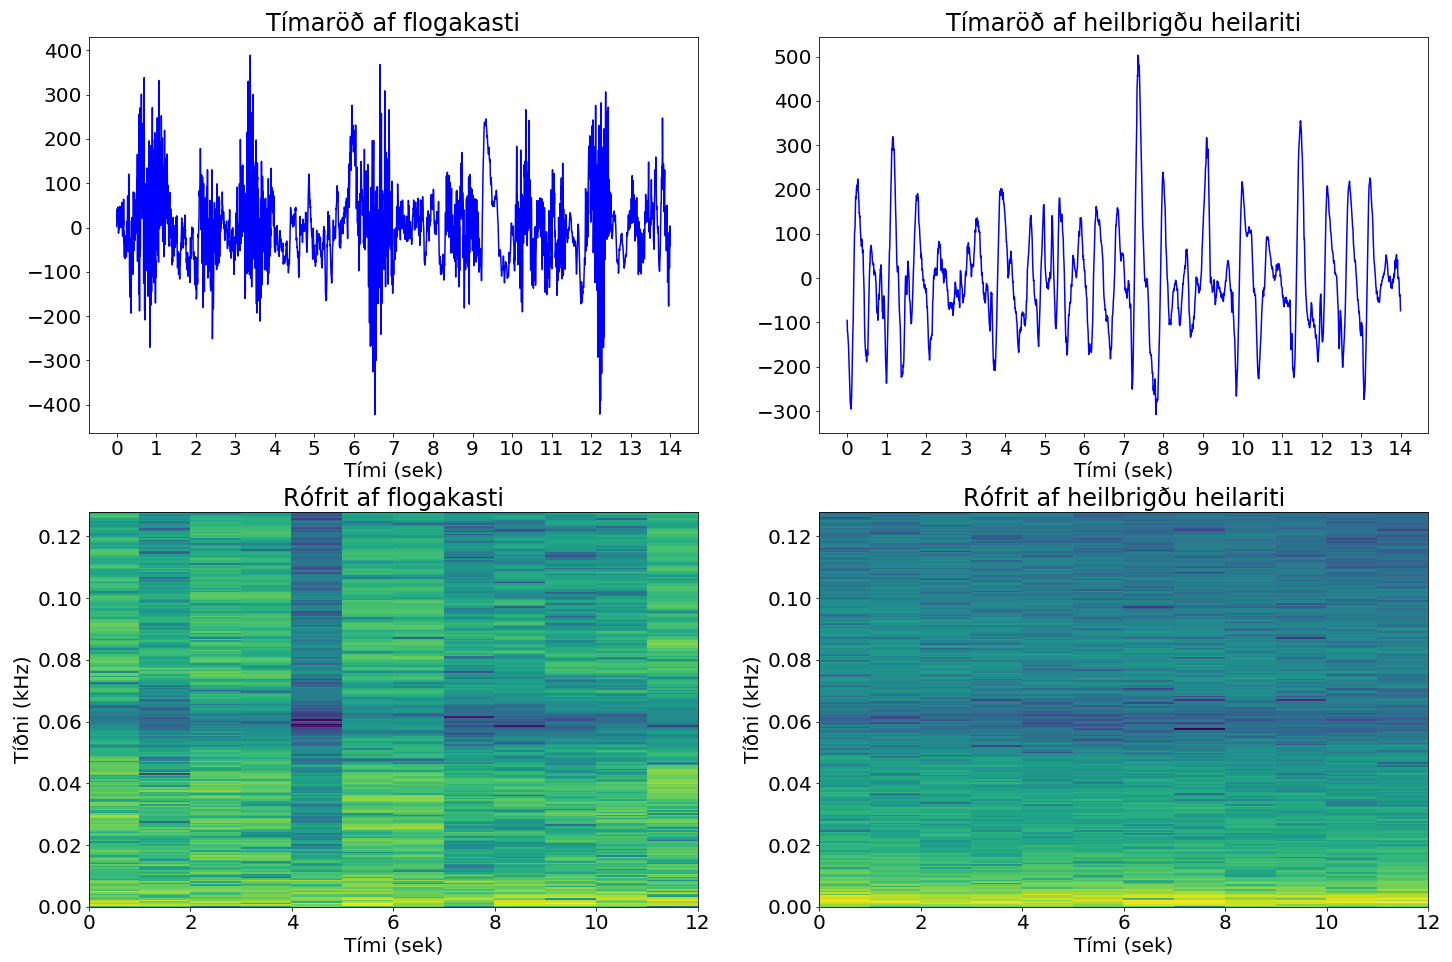
\includegraphics[width = \textwidth]{rofrit.png}
    \caption{Tímaraðir og Rófrit}
    \label{rofrit}
\end{figure}

Með því að umbreyta sérhverri tímaröð í rófrit þá getum við litið svo á að hvert af okkar 540 tilvikum hefur eina 23 laga mynd þar sem hvert lag er rófrit úr einni rás. Þessar myndir getum við notað til að þjálfa földunartauganet. 
Földunarnet hafa hvert sinn strúktúr, þ.e. hversu mörg hulin lög það hefur, hversu marga hnúta, hversu stóran földunarglugga o.s.frv. Við prófuðum ýmis mismunandi strúktúra sem virkuðu misvel. Við bárum saman strúktúrana með tilliti til prófunarnákvæmni, prófunartapi, næmi og sértækni. Í þjálfuninni fylgjumst við með prófunartapinu og ef það batnar ekki í þrjú tímabil (e. epochs) í röð þá hættum við þjálfuninni og sættum okkur við núverandi líkan. Gagnasettið hér er ekki voða stórt, hvert inntak er fremur stórt (cirka $256\times 14 \times 23$ víð mynd) en við höfum aðeins 540 inntök. Tauganet virka best ef fyrirliggur stórt gagnasett, því er líklegt að við munum ofmáta tauganetið. 

\subsection{Einstaklingsmiðuð greining}
Eftir að hafa borið saman flokkarana á öllu gagnasafninu þá völdum við þann besta og athuguðum hvernig hann stóð sig í því að greina einn einstakling í einu. Gögnunum var þá skipt niður eftir einstaklingum, flokkarinn þjálfaður á öllum einstaklingum nema einum og svo prófaður á öllum tilvikum þess einstaklings. Nákvæmni, sértækni og næmi flokkarans voru reiknuð og svo allt endurtekið fyrir hvern einstakling. Einstaklingarnir hafa mismargar mælingar og mismörg tilvik af flogaköstum. 
\section{Niðurstöður}

\subsection{Grindarleit}
Framkvæmd er grindarleit (e. grid search) á þremur flokkurum {\tt SVM}, {\tt Adaboost} og {\tt Logistic regression} í þeim tilgangi að finna þá yfirstika sem skila bestu prófunarnákvæmni ásamt næmi og sértækni.
\label{ch:grindarleit}
\begin{figure}[H]
    \centering
    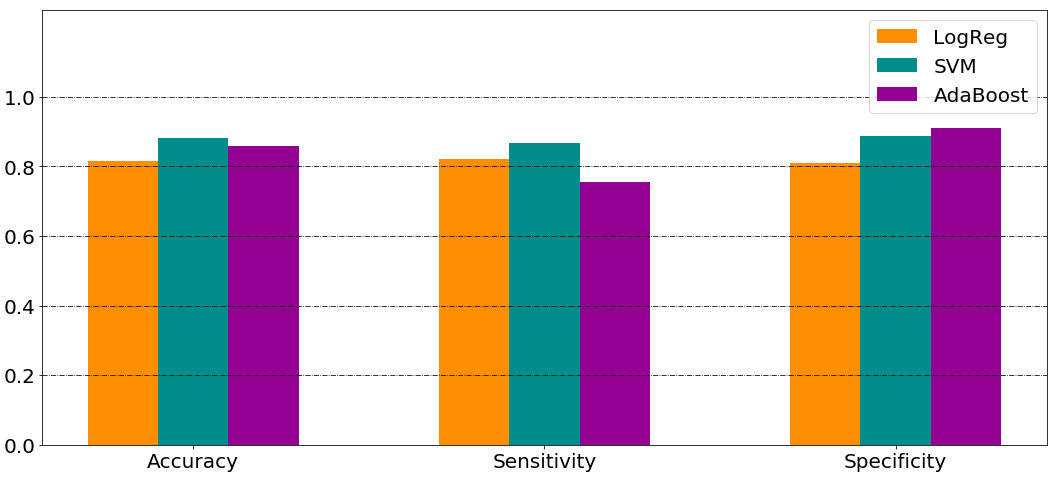
\includegraphics[width=\textwidth]{Gridsearch.png}
    \caption{Samanburður á prófunarnákvæmni, næmi og sértækni fyrir flokkarana með sínum bestu yfirstikum fyrir stærð tímarammans sem 14 sekúndur, Fáum eftirfarandi stika {\tt LogReg:} $C=20$; {\tt SVM:} $C=8$, $\gamma = 0.0015$; {\tt AdaBoost:} learning\_rate=0.5, n\_estimators=150} 
    \label{fig:Gridsearch}
\end{figure}

Við sjáum að stoðvigravél stendur sig best á þeim vígvöllum sem við höfum helstan áhuga á, prófunarnákvæmni og næmi. Við ákveðum því að stoðvigravél með þá yfirstika sem ákvarðaðir voru með grindarleitinni ($C = 8$ og $\gamma = 0.0015$) sé besti flokkarinn fyrir okkar verkefni. Við skoðuðum næst hvernig mismunandi stærð á tímarömmum hefur áhrif á flokkarann.
\subsection{Tímarammi}
Við skoðuðum alla mögulega tímaramma og mátuðum stoðvigravélina okkar við samsvarandi gögn og reiknuðum lýsistærðirnar fyrir hvern tímaramma. Niðurstöðurnar má sjá hér að neðan í mynd \ref{fig:tlength}.

\begin{figure}[H]
    \centering
    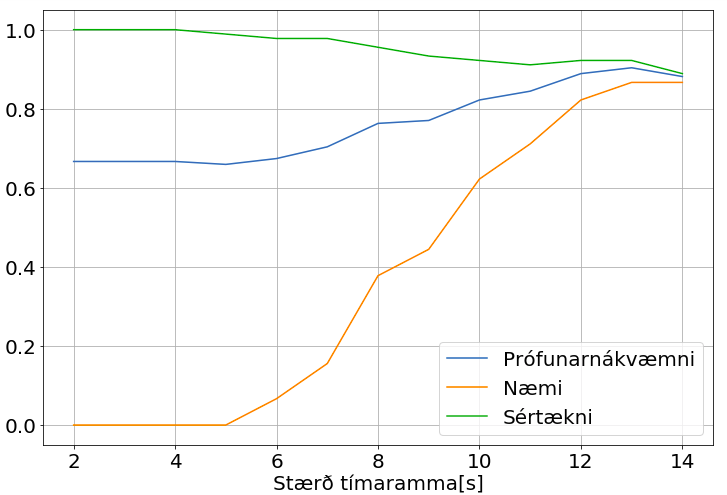
\includegraphics[width=0.7\textwidth]{SVMtime.png}
    \caption{Prófunarnákvæmni, næmi og sértækni stoðvigravéla sem fall af stærð tímaramma. Notað er stoðvigravél með yfirstika $C=8$ og $\gamma=0.0015$}
    \label{fig:tlength}
\end{figure}
Við höfum mestan áhuga á prófunarnákvæmni og næmi og sjáum að við fáum hágildi á þeim stærðum þegar stærð tímarammans er í 13 sekúndum. Þegar stærð tímarammans er 13 sekúndur fáum við 90.37\% í prófunarnákvæmni, 86.67\% í næmi og 92.22\% í sértækni sem er ágætlega gott. \\

Með réttu yfirstika og rétta stærð af tímaramma þá höfum við sætt okkur við lokaflokkarann okkar og mynd \ref{svm_cm} hér að neðan sýnir ruglingsfylki hans.

\begin{figure}[H]
    \centering
    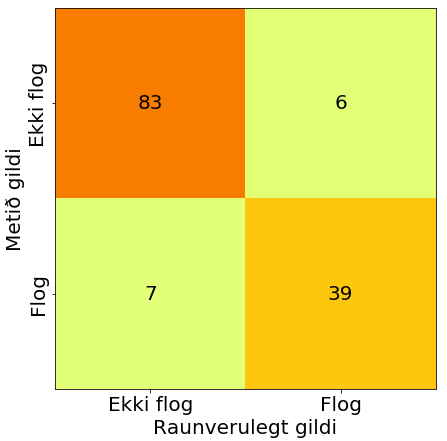
\includegraphics[width=0.45\textwidth]{svm_cm.png}
    \caption{Ruglingsfylki Stoðvigravélarinnar}
    \label{svm_cm}
\end{figure}

Þessi niðurstaða er vel ásættanleg, við athugum nú hvernig þessi flokkari hagar sér þegar hann greinir einn einstakling í einu.

\subsection{Einstaklingsmiðuð greining}
Hér á mynd \ref{patspec_svm} má sjá hvernig útvaldi flokkarinn okkar stóð sig í því að greina heilarit hvers einstaklings fyrir sig.

\begin{figure}[h]
    \centering
    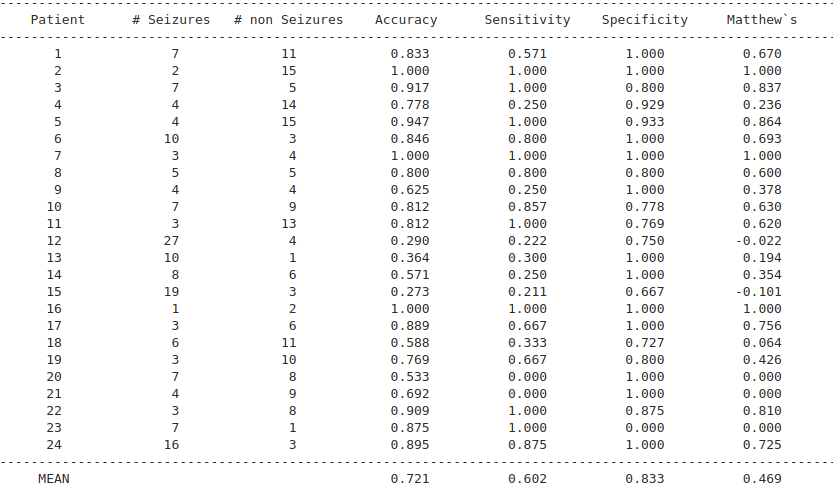
\includegraphics[width = \textwidth]{patspec_svm.png}
    \caption{Einstaklingsmiðuð greining stoðvigravélarinnar}
    \label{patspec_svm}
\end{figure}

Niðurstöðurnar eru ekki eins góðar og við vonuðumst eftir. Við náum aðeins 72.1\% meðalprófunarnákvæmni og aðeins 60.2\% meðalnæmi. Þetta telst alls ekki nógu gott til þess að nýta flokkarann fyrir alvöru. Með rýnun í töfluna að ofan má sjá að oft vill flokkarinn bara giska á annan flokkinn alltaf. Ástæðuna fyrir þessari lélegu frammistöðu má líklega rekja til skölunar á gögnunum. Nú eru stoðvigravélar mjög næmar fyrir skölun og gögnin hafa mikla dreifni svo skölunin getur verið mismunandi eftir því hvert þjálfunarsafnið er og þessir fáu prófunarpunktar gætu skalast furðulega. Við prófuðum bæði að sleppa sköluninni og breyta yfir í MinMax skölun en það skilaði aðeins verri niðurstöðum. Einnig voru hinir flokkararnir, lógistíska aðhvarfsgreiningin og AdaBoost með bestu yfirstikunum úr grindarleitinni prófaðir en þeir skiluðu einnig verri niðurstöðum.

\subsection{Tauganet}
Eftir margar prófanir á mismunandi strúktúrum földunarnetsins þá enduðum við að vinna með eftirfarandi strúktúr sem má sjá á mynd \ref{Tauganet_sktruktur}.

\begin{figure}[h]
    \centering
    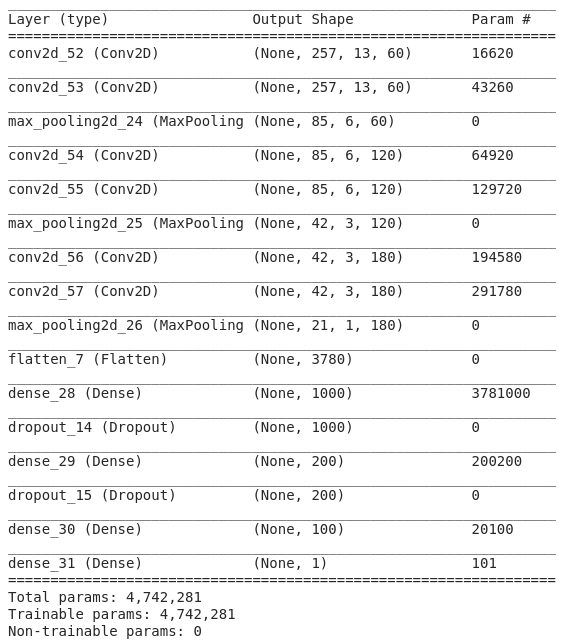
\includegraphics[width = 0.7\textwidth]{Tauganet_86_struktur.png}
    \caption{Strúktúr Tauganetsins}
    \label{Tauganet_sktruktur}
\end{figure}

Í orðum þá byrjuðum við á tveimur 60 hnúta földunarlögum með földunarglugga að stærð $6\times 2$, ástæðan fyrir þessari afbrigðilegu gluggastærð er að upphaflegu myndirnar okkar eru $257\times 13$ að stærð svo við viljum safna upplýsingum um fleiri tíðnibil á þrengri tímabilum. Eftir fyrstu földunarlögin kemur safnlag með $2\times 2$ glugga, tvö 120 hnúta földunarlög með $3\times 3$ glugga, safnlag, tvö 180 hnúta földunarlög, safnlag og svo þrjú full tengd lög með 1000, 200 og 100 hnútum með úrfellingum á milli. \\
Þetta tauganet náði prófunarnákvæmni upp á $86.7\%$ og tap upp á $0.3033$ eftir að hafa lært í 11 tímabil (e. epochs) en yfirlit um þjálfunarsögu netsins má sjá á mynd \ref{Tauganet_history}.

\begin{figure}[H]
    \centering
    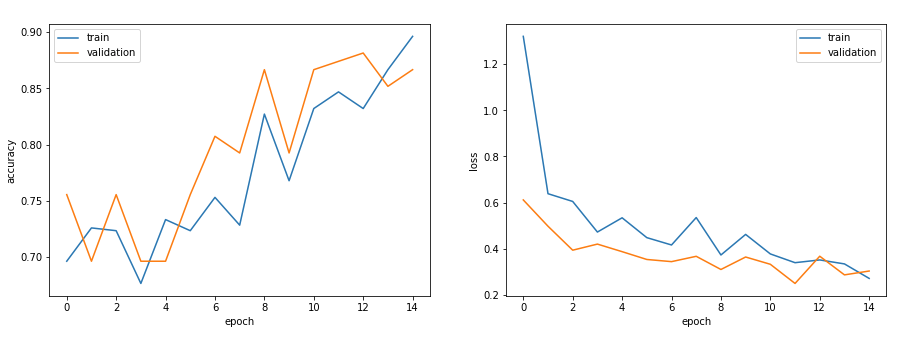
\includegraphics[width=\textwidth, height = 0.25\textheight]{Tauganet_86_history.png}
    \caption{Lærdómur Tauganetsins, nákvæmni til vinstri og tap til hægri}
    \label{Tauganet_history}
\end{figure}

Nákvæmnin flöktar heldur mikið sem er eðlilegt með svo lítið gagnasett en tapið hegðar sér fremur vel. Við sjáum svo ruglingsfylki tauganetsins hér að neðan á mynd \ref{Tauganet_cm}.

\begin{figure}[H]
    \centering
    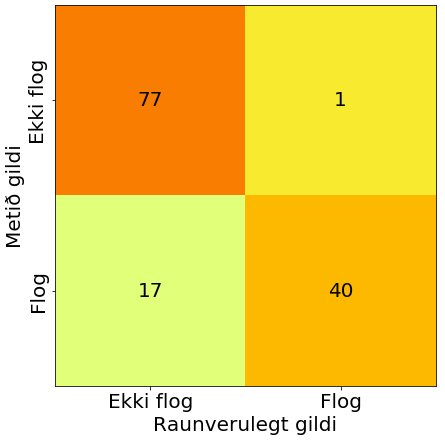
\includegraphics[width=0.45\textwidth]{Tauganet_86_cm.png}
    \caption{Ruglingsfylki Tauganetsins}
    \label{Tauganet_cm}
\end{figure}

Eins og nefnt er hér að ofan þá er næmi mikilvægasta lýsistærðin okkar og tauganetið náði næmi upp á $97.56\%$, sem er frábært. Við sjáum af ruglingsfylkinu hér að ofan að það er aðeins eitt tilvik þar sem tauganetið missir af flogakasti. Þrátt fyrir þessa háu næmi þá borgum við ekki stórt gjald í sértækninni á móti því hún er upp á $81.91\%$, Matthew stuðullinn er upp á $0.74$ sem er ágætt sérstaklega fyrir svona háa næmi. \\
\\

Við prófuðum að nota tauganetið okkar sem einstaklingsmiðaðann flokkara en það fór ekki vel, meðal nákvæmnin endaði í $60.6\%$, næmnin í $45.7\%$ og sértæknin í $65.2\%$. Svo virtist sem tauganetið hallaðist að því að giska alltaf á ekki flog. 
\section{Samantekt}
Okkur hefur tekist að smíða tvo ólíka flokkara, stoðvigravél og földunarnet, sem nema flogaköst í heilaritum með annars vegar 90.37\% prófunarnákvæmni og 86.67\% næmi með stoðvigravélinni og hins vegar $86.7\%$ prófunarnákvæmni og $97.56\%$ næmi með tauganetinu. Flokkararnir tveir notuðu ólík auðkenni sem inntaksgögn sem þó bæði byggðu á tíðni- og tímaupplýsingum. Hægt er að vinna önnur auðkenni úr tímaröðum og mögulegt er að þau skili betri árangri í flokkun en gert var hér. Bæði stoðvigravélin og tauganetið stóðu sig leiðinlega illa í því að greina einstaklingsbundin flogaköst, enda er það erfitt verk því flogaköst eiga það til að koma ólíkt fram hjá ólíku fólki. Það er því eitthvað sem þyrfti að leggja betri áherslu á í áframhaldandi vinnslu á þessu verkefni.
\bibliographystyle{siam}
\bibliography{bibtex}
\end{document}
